%\documentclass[twocolumn]{article}
\documentclass{article}
\usepackage{outline}
\usepackage{float}
\usepackage{graphicx}
\usepackage{color}
\usepackage{amsmath}

%% The following should allow me to make subsubsubsections with the command \paragraph{}
\usepackage{titlesec}

\setcounter{secnumdepth}{4}

\titleformat{\paragraph}
{\normalfont\normalsize\bfseries}{\theparagraph}{1em}{}
\titlespacing*{\paragraph}
{0pt}{3.25ex plus 1ex minus .2ex}{1.5ex plus .2ex}
%%

\graphicspath{ {Figs/} }

\begin{document}

 \title{Multiscale Modeling of the Paradoxical Roles of the Immune System in EMT-Mediated Cancer}
 \maketitle

\section{Abstract}
%% Basic Introduction (1-2 sentences)
During tumorigenesis and throughout the lifetime of a tumor, the immune system is constantly engaged in complex interactions in and around the tumor.
%% More Detailed Background (2-3 sentences)
These interactions are influenced by the tumor microenvironment (TME) and in particular by the cellular process of epithelial-to-mesenchymal transition (EMT) in an as-yet unexplained manner.
In turn, both the tumor and the immune system exert substantial influence over the TME in competition to influence the fate of the host.
%% General Problem (1 sentence)
Determining the critical factors and mechanisms involved remains a crucial task for cancer immunotherapy.
%% Summarizing Main Result (1 sentence)
Here, we seek to understand how interplay between the tumor, the immune system, and EMT can determine the outcome of cancer.
%% The Main Result (2-3 sentences)
We developed a multiscale agent-based model that describes tumor-immune interactions and how EMT modulates these.
Exploration of the model revealed that increasing mesenchymal cells' quiescence in some circumstances results in a more tumor-friendly environment and sometimes less.
In contrast, enhancing mesenchymal cells' immune evasiveness always leads to a more tumor-friendly microenvironment.
Moreover, encouraging the TME towards a pro-EMT state also benefits the tumor.
%% Putting into a More General Context (1-2 sentences)
Together, these results indicate that the joint regulation of the TME by the immune system and the tumor itself provides possible targets for future cancer therapies, in particular cancers such as pancreatic cancer in which EMT is speculated to play a role.

%%%%%%%%%%%%%%%%%%%%%%%
%                    INTRODUCTION                    %
%%%%%%%%%%%%%%%%%%%%%%%

\section{Introduction}
Immunotherapy is revolutionizing cancer therapy.
Year-by-year, more breakthroughs in the field produce effective new drugs and therapies that are having a significant impact on patient health and survival.
This is an exciting and fast-paced time in the field and many believe it just the beginning.
There are myriad untapped avenues by which scientists can further explore the role of the immune system in regulating and combatting cancer.
While the direct cell-cell interactions between immune cells and cancer cells is an unsurprising line of inquiry, how immune cells interact with and modulate the tumor microenvironment (TME) is also a promising lead.

This is because immune cells are best understood as one constituent of the TME: responding to the environment's inflammatory signals, fighting the mutated cells present, and then restoring homeostasis in that local context.
Understanding each step in this immune cascade in the context of the TME will be paramount in fully exploring and exploiting all options for immunotherapy.

One aspect of the TME long suspected of playing a vital role in tumor initiation, progression, and metastasis is the epithelial-to-mesenchymal transition (EMT). 
This is the process by which rigidly bound epithelial cells leave a layer of cells and gain motility as mesenchymal cells, among other properties.
As mesenchymal cells often express stem-like properties, their existence has been tied to the initiation and progression of cancer.
Also, due to their motility, some have viewed them as a natural precursor to metastasis.

Thus, herein we explore the interconnectedness of these three features: the tumor itself, the immune system, and the EMT process.
In addition to the interactions already mentioned above, the immune system also affects and is affected by EMT.
The immune system affects EMT by releasing a flurry of cytokines upon arrival in the TME.
In particular, regulatory T cells (Tregs) release copious quantities of the EMT-driving transforming growth factor beta (TGF-$\beta$).
Conversely, the EMTed cells in the tumor downregulate certain surface markers making it more difficult for cytotoxic immune cells to form the immune synapse necessary to lyse the cancer cell.

Taking these three aspects together, all influencing the others, we can consider the simple diagram in Figure \ref{fig:3PartFig} and see just how much potential there is for exploring all these relationships.
Each of these three pieces will be briefly explored in turn for how they will influence one another.

\subsection{The Tumor}\label{TheTumor}
The tumor influences the immune system by its presence and by the cellular processes it engages in that result in shaping the TME.
On the one hand, the mutated DNA of tumor cells results in these cells being recognized as foreign by members of the innate immune system such as Natural Killer cells and Dendritic cells.
It is then these cells that initiate the cascade of cytokines that result in the full activation of the body's immune system to fight the non-self cells.
On the other hand, the tumor cells actively work to shape the immune response that the body launches.
This is accomplished through its own set of cytokines, such as TGF-$\beta$, that work to create a tumor-supportive environment, including shifting the immune balance to be immunosuppressive by enhancing the recruitment of Treg cells.

As mentioned above, TGF-$\beta$ is one driver of EMT, and so it is through direct release of TGF-$\beta$ and recruitment of TGF-$\beta$-secreting Treg cells that the tumor encourages itself and the surrounding tissue towards a more mesenchymal profile. 

\subsection{The Immune System}\label{TheImmuneSystem}
The immune system has several competing interactions with the tumor.
While the cytotoxic immune cells, NKs and CTLs, seek out and lyse tumor cells, the regulatory branch of the immune system, Tregs, slows down the effector functions of these other cells.

These Tregs also drive the EMT process by releasing TGF-$\beta$ upon arriving at the tumor site.

\subsection{EMT}\label{EMT}
There are many characteristics distinctive of mesenchymal cells and still much research being done in further quantifying these and determining others.
Of interest here, the literature shows two qualities of mesenchymal cells that are of interest particularly in the context of cancer and the immune system.
The first is that mesenchymal cells are less susceptible to immune clearance.
The second is that mesenchymal cells proliferate at a slower rate.

The research on mesenchymal cells' immune evasiveness is quite conclusive with the research even going so far as establishing functional causes for this phenomenon.
Once cytotoxic immune cells, for example natural killer cells and cytotoxic T cells, have targeted a cell to lyse, they necessarily must make a physical connection with that cell, termed an immunological synapse.
However, due to down-regulated surface markers on mesenchymal cells, they are refractory to this immunological task thus rendering them less susceptible to immune clearance.
In line with known motility of mesenchymal cells, scientists have referred to this condition as mesenchymal cells being ``slippery.''
This quality of mesenchymal cells is then quantified in our model by the parameter, MIE, for mesenchymal immune evasion.

The other facet of mesenchymal cells of importance in this research is their slower proliferation rate, and this is tied to the observation that mesenchymal cells often express a more stem-like phenotype.
Indeed, even in healthy tissue, this is readily observed and seen as a useful mechanism for homeostasis as epithelial cells can transition to mesenchymal, stem-like cells under appropriate conditions.
While many qualities are associated with being stem-like, we choose to focus on a reduced proliferation rate.
In quantifying this property, we use the model parameter, MQ, for mesenchymal quiescence.
This choice is less about associating this property with quiescence and more about creating a simple name that easily, if not roughly, captures the essence of what is being modeled.
For example, while mesenchymal proliferation reduction might be a more accurate term, thinking in terms of a negative formulation adds one additional twist to accurately interpreting results which we felt was more detrimental than the possible confusion of invoking ``quiescence.''


%%%%%%%%%%%%%%%%%%%%%%%
%                         METHODS                        %
%%%%%%%%%%%%%%%%%%%%%%%

\section{Methods}
To address the questions around the relationships among cancer, the immune system, and EMT, we built a multiscale, agent-based model to explore.
The agents in the model are the tissue cells that can either be healthy or have mutations.
It is worth noting that unlike many agent-based models, the spatial arrangement of these cells is not part of the model.
Thus, it is assumed that all the cells are in effect well-mixed as are all the relevant cytokines and other molecules acting on the system.
The immune cells are present in aggregate, i.e. only the total quantity of them present in the tumor microenvironment (TME) is used.
Finally, it is the tissue cells that can be labeled either epithelial or mesenchymal, and this labeling is fluid and depends both on the TME and the internal workings of each individual cell.

\subsection{Tissue Cells}\label{TissueCells}
The tissue cells at all times have associated with them two important quantities: a logical vector indicating pathway mutations and an EMT score.
The model has three pathways that have the potential to mutate over the course of a simulation.
There is a proliferation pathway that when mutated increases the probability of the cell proliferating.
There is an apoptosis pathway that when mutated decreases the probability of the cell undergoing apoptosis.
There is an immune evasion pathway that when mutated decreases the probability that an immune cell can effectively clear the mutated cell.
% It might be nice to have a table to summarize this information?
The EMT score will be exposited in Section \ref{EMT}.

Add differential equations? % Adam suggested this, but I'm not sure what this means.
\subsection{The Immune System}\label{ImmuneSystem}
The immune system is modeled as having three active immune cell types: Natural Killer cells (NKs), cytotoxic T cells (CTLs), and T regulatory cells (Tregs).
The NKs and CTLs act on the system by recognizing mutated cells and clearing them.
Should they clear a cell, they themselves are then deactivated and removed from the immune population.
Tregs act on the system by suppressing the effector functions of NKs and CTLs, making it less likely they can clear mutated cells.
In addition to this, Tregs release TGF-$\beta$ which further shapes the TME by pushing tissues cells more towards a mesenchymal phenotype.

\subsection{EMT}\label{EMT}
The EMT score indicates how likely the cell is begin the next cell cycle as an epithelial or a mesenchymal cell.\
The score is between $0$ and $1$ with higher values being connected to higher probability of being mesenchymal.
For each patient, there is a fixed mesenchymal threshold.
If the EMT score ends the cycle above this threshold, the cell is mesenchymal, otherwise it is epithelial for the next cycle.
For the purposes of the model, a cell in an epithelial state is considered in the base state, and one in a mesenchymal state will have some of its parameters updated.
In particular, mesenchymal cells benefit from increased immune evasion but suffer from decreased proliferation.
Note, that because the immune system can only clear mutated cells, the increased immune evasion only benefits mutated mesenchymal cells.

\subsection{Running the Model}

\subsubsection{Initializing the Model}
Every model run starts with a fixed amount of cells, $N_0$.
However, different parameter values will lead to different steady states for the population of tissue cells.
In light of this, a warmup period of ~1000 cell cycles is used in which time no mutations are allowed to happen.
Thus, the only immune cell present is NKs.
After the warmup cycles are complete, a mutagenic event is simulated in which all the tissue cells experience a discrete, random jump in their probability to mutate.
From then on, a cell which proliferates either mutates or increases its probability of mutating later on.

\subsubsection{Cell Fate}
During each cell cycle, every cell randomly is assigned a cell fate from the following options:
\begin{itemize}
\item proliferation
\item apoptosis
\item immune clearance (by NKs or CTLs)
\item quiescence
\end{itemize}

For each cell, a weight is chosen for each option and these are normalized to probabilities which then are used to randomly determine what each cell does during the cell cycle.

\paragraph{Proliferation}
There are four factors that contribute to a cell's probability to weight.
The first is a base proliferation weight that all cells have, $p$.
Second, if the cell has a mutation in the proliferation pathway, then the weight for proliferation is proportionally increased by $\text{prolif}_{\text{up}}$.
Third, if the cell is mesenchymal, then the weight for proliferation is proportionally decreased by $m_Q$, which stands for mesenchymal quiescence.
Fourth, there is a negative feedback of the cells on their own proliferation which is quantified by a Hill factor.
In total, the weight for proliferation is given by

$$ p_{\text{prolif}} = p(1+\delta_{\text{PM}}\text{prolif}_{\text{up}})(1-\delta_{MES}m_Q)\frac{N_0}{N_0+N} $$

\paragraph{Apoptosis}
There are two factors that contribute to a cell's weight for undergoing apoptosis.
There is a basal apoptosis rate that all cells experience, $d$ for death.
Second, if the cell has a mutation in the apoptosis pathway, then the weight for undergoing apoptosis is proportionally decreased by $\text{apop}_{\text{down}}$.
In total, the weight for apoptosis is given by 

$$ p_{\text{apop}} = d(1-\delta_{\text{AM}}\text{apop}_{\text{down}}) $$

\paragraph{Immune Clearance}
For both NK clearance and CTL clearance, the weights are built with the same factors but have different parameter values for NK and CTLs.
First of all, the cell needs to be mutated, $\delta_M$.
Second, there is a Hill factor that captures the probability of an immune cell finding and interacting with the given tissue cell.
Third, NKs and CTLs have their own efficacy parameters which can be understood as their probability of clearing a mutated cell given that they have interacted with it.
Fourth, there is a decreasing Hill factor based on the number of Treg cells present.
Finally, there are two factors that proportionally decrease the weight of immune clearance depending on if the cell has an immune evasion mutation or if it is mesenchymal.
In total, the weight of NK clearance is given by

$$ p_{\text{NKed}} =  \delta_M \frac{\text{NK}}{N/N_{00}+\text{NK}} E_{\text{NK}} \frac{1}{1+\text{Treg}/\text{Treg}_{\text{EC50}}} $$ $$ (1-\delta_{IEM}\text{IE}_{\text{up}})(1-\delta_{MES}m_{\text{IE}})$$

A similar formula holds for CTLs with only the number of CTLs and their efficacy being different from the above equation.


\paragraph{Quiescence}
The weight associated with quiescence is taken as 1 except in the case of Mesenchymal cells.
For Mesenchymal cells, the weight lost to proliferation is added to the weight of quiescence.
Hence, the weight of quiescence is given by

$$ p_Q = 1 + \delta_{\text{MES}}p(1+\delta_{\text{PM}}\text{prolif}_{\text{up}})m_Q\frac{N_0}{N_0+N} $$

The reason for adding that term is due to the understanding that mesenchymal cells are not proliferating as fast because they are instead remaining quiescent, hence naming the parameter $m_Q$.

\subsubsection{Completing the Cell Cycle}
After the cell fates are determined and the results reflected in the system, there are a few things that happen before the system moves on to a new cell cycle.
First, the NK and CTL populations are reduced by the number of mutated cells they cleared.
This represents the fact that individual immune cells have a limited amount of efficacy.

Also, all proliferating cells have a probability of undergoing a pathway mutation.
If they do, one is randomly chosen among the three and that one either mutates or remains mutated.
If they do not mutate, then their probability of mutating increases.

Then, the EMT values for each cell is updated.
This depends on how much TGF-$\beta$ is currently in the system.
Each cell receives an amount of TGF-$\beta$ given by

$$ \text{TGFB}_i = \text{TGFB}/N + X_i, \quad X_i \sim N(0,\sigma^2)  $$

where $\sigma$ is a parameter in the model.
This quantity is then compared to $2-\text{EMT}_i$ where $\text{EMT}_i$ is the EMT score of the $i^{th}$ cell on a scale of $[0,1]$ with $0$ representing most epithelial and $1$ representing most mesenchymal.
If $\text{TGFB}_i>2-\text{EMT}_i$, the cell is EMTed and will have a higher EMT score.
If $\text{TGFB}_i<2-\text{EMT}_i$, the cell is METed and will have a lower EMT score.
The reason for the expression $2-\text{EMT}_i$ can be understood this way: 
the bounds on the EMT score guarantee $2-\text{EMT}_i\in[1,2]$.
Hence, there either needs to be a lot of TGF-$\beta$ in the system or a large amount of randomness for a cell to undergo EMT.
In addition, a cell having a higher EMT score will have a higher chance of continuing in the EMT process whereas a cell low on the EMT spectrum will have a higher chance of moving towards a more epithelial phenotype.

Next, the amount of TGF-$\beta$ for the next cell cycle is determined by the number of mutated cells and the number of Treg cells, each one producing a fixed amount of TGF-$\beta$. It is given by

$$ \text{TGFB} = \text{tgfb}_{\text{mut}}N_{\text{mut}} + \text{tgfb}_{\text{Treg}}\text{Treg}$$

Finally, the immune populations are updated.
For the NKs, they obey the following differential equation:
 
$$ \text{NK}' = \sigma_{\text{NK}} - d_{\text{NK}}\text{NK} $$

which is discretized to

$$ \text{NK}_{i+1} = \left (\text{NK}_i-\frac{\sigma_{\text{NK}}}{d_{\text{NK}}} \right )\exp(-d_{\text{NK}}\Delta t)+\frac{\sigma_{\text{NK}}}{d_{\text{NK}}} $$

For CTLs and Tregs, however, they rely on antigen presenting cells (APCs) to be activated, and these APCs in turn rely on mutated cells being cleared so that they can bind antigens.
In addition, Treg recruitment is upregulated by TGF-$\beta$, which will be incorporated via a Hill function.
Thus, let $\text{APC}$ represent the number of mutated cells cleared by the immune system during a given cycle.
We choose the following differential equations to govern the CTL and Treg populations:

\begin{align*}
\text{CTL}' & = \sigma_{\text{CTL}}\text{APC} - d_{\text{CTL}}\text{CTL} \\
\text{Treg}' & = \sigma_{\text{Treg}}\text{APC} \frac{\text{TGFB}}{1+\text{TGFB}/\text{EC50}}- d_{\text{Treg}}\text{Treg}
\end{align*}

Discretized, these are:

\begin{align*}
\text{CTL}_{i+1} & = & \left (\text{CTL}_i-\sigma_{\text{CTL}}\text{APC}/d_{\text{CTL}}\right )\exp(- d_{\text{CTL}}\Delta t) + \sigma_{\text{CTL}}\text{APC}/d_{\text{CTL}}\\
\text{Treg}_{i+1} & = & \left (\text{Treg}_i-\frac{\sigma_{\text{Treg}}\text{APC}}{d_{\text{Treg}}} \frac{\text{TGFB}}{1+\text{TGFB}/\text{EC50}}\right )\exp(-d_{\text{Treg}}\text{Treg}\Delta t)+\\
& & \frac{\sigma_{\text{Treg}}\text{APC}}{d_{\text{Treg}}} \frac{\text{TGFB}}{1+\text{TGFB}/\text{EC50}}
\end{align*}

\subsubsection{Cancer Onset}
At the end of each cell cycle, the proportion of tissue cells that are mutated is checked, and if it is above a certain threshold the patient is determined to have developed cancer and a Time to Cancer is recorded.
If not, the process continues until cancer is detected or a preset number of cycles has been completed.
It is also possible with the right combination of parameters, to have patients run out of cells entirely.
The model does not distinguish between these patients and those that have a cancer diagnosis.
The reason is that these patients have succumb to some combination of inflammatory and mutagenic events.

%%%%%%%%%%%%%%%%%%%%%%%
%                          RESULTS                         %
%%%%%%%%%%%%%%%%%%%%%%%

\section{Results}

\begin{figure}[H]
\center
\frame{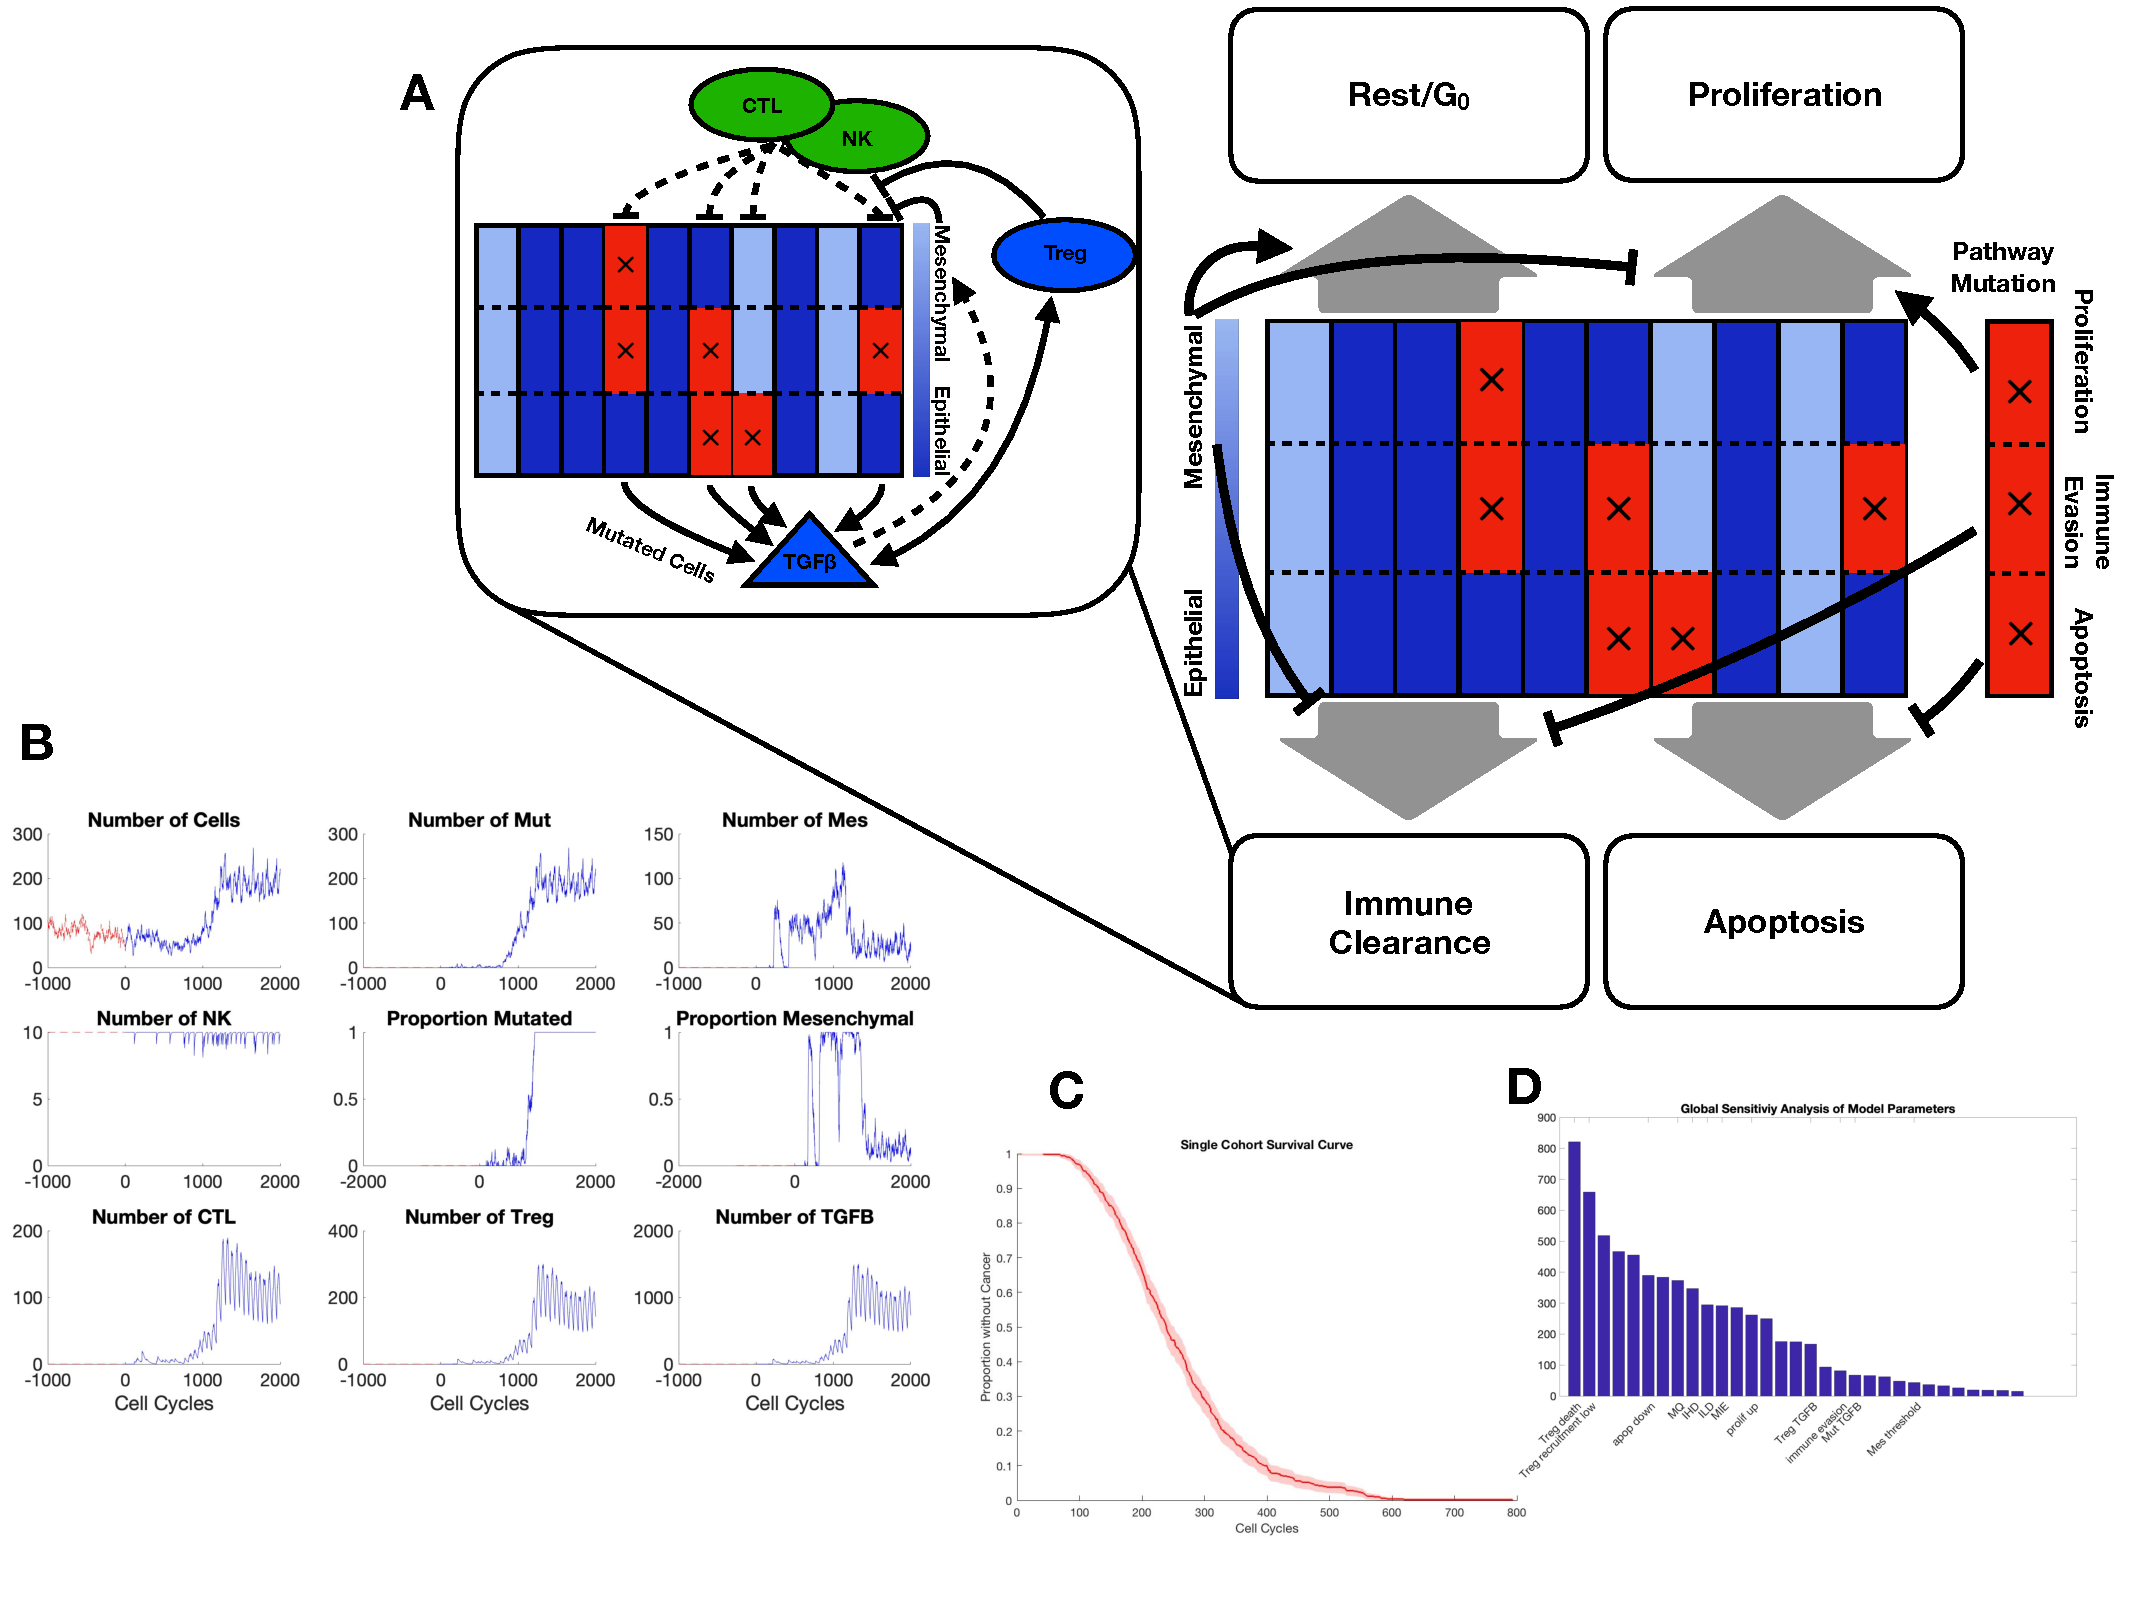
\includegraphics[width=\columnwidth]{Figure1/Figure1.pdf}}
\caption{A. A cartoon of the cell cycle with the immune system interactions as an inset.
B. Global sensitivity analysis.
C. Example survival curve for one cohort.
D. Example of one simulated patient's dynamics. The warmup period for the model is plotted in red.}
\label{fig:ModelIntro}
\end{figure}

\subsection{Exploring the Model}\label{ExplModel}
Refer to Figure \ref{fig:ModelIntro}A for a cartoon of the model.
Here, each cell is represented as a column with three components representing the three possible mutations a cell can have.
If the component is red and has an `X' in the middle, then that indicates the cell has undergone a pathway mutation corresponding to the example cell on the right.
If any component of a cell has a pathway mutation, that cell is then counted as a mutated cell and contributes towards the total number of cancer cells.
Each cell also has a color along the EMT spectrum seen on the left of the cell block. 
Biologically, cells can be anywhere along this continuum with research indicating there are several equilibria along the spectrum.
In our model, this is actually just a binary and that is why the cells shown are at one extreme or the other of the spectrum.

In the right half of Figure \ref{fig:ModelIntro}A one can see the cell cycle choices that each cell can make each cell cycle.
These are the four thick, gray arrows.
Each of the cells will choose which arrow to follow each cell cycle, and this decision is influenced by the properties of the cell as well as external factors like the immune system and the TME.
The inset on the left gives an overview of how the immune system works.
The dashed arrows indicate that the action is probabilistic rather than deterministic.
In other words, the cytotoxic cells will randomly clear some subset of mutated cells and TGF-$\beta$ increases the probability of cell transitioning or staying in a mesenchymal state.

For a typical {\it in silico} patient, see Figure \ref{fig:ModelIntro}B.
Notice that at cell cycle number 541 the proportion of mutated cells reaches 50\% and so the patient has a Time to Cancer of 541.
Once the Time to Cancer has been determined for a patient, most simulations shown later stop.
We do this because once such a high proportion of cells have mutated, the mutant cells quickly take over and make up 100\% of all cells.
Also of interest, as the patient's cells are all rapidly mutating right around this time, most of them are also transitioning to a mesenchymal phenotype with all of them being in a mesenchymal phenotype for a short time during the time period that cancer onset occurs.

Considering the immune populations, notice that the NK population basically stays constant while the lymphocyte populations quickly dwarf the NK population once cells begin to mutate.
These lymphocyte populations exhibit oscillatory behavior but this is an artifact of the inflammation scheme this patient is undergoing.
Every 30 cell cycles the inflammation changes from High to Low or vice versa.
In these roughly month-long periods, the lymphocyte populations increase or decrease rapidly in accordance with this inflammation.

Finally, considering a cohort of $N=500$ patients, we can generate a survival curve for these patients tracking how many have survived cancer-free up to a give day.
See Figure \ref{fig:ModelIntro}C for such a survival curve.
In this curve, we see that all patients survive for some minimum amount of time before a time period a nearly constant cancer onset rate roughly between $T = 100$ and $T = 300$.

\subsection{Sensitivity Analysis}\label{SensAnalysis}
To assess the sensitivity to the many model parameters, a Morris OAT algorithm was implemented.
The parameters were all given Gaussian distributions centered at their initial value and a large standard deviation.
Those that needed bounds were truncated.
The results of the Morris OAT can be found in Figure \ref{fig:ModelIntro}D.
Clearly, a certain subset of parameters have an outsized effect on the model while others do relatively little.
The two most influential according to this analysis are related to Treg cells: their death rate and recruitment.
This makes sense as Treg cells both suppress cytotoxic effects of other immune cells and also secrete significant quantities of TGF-$\beta$ which drives EMT.
Thus, Treg cells are intimately tied to all three aspects of the model and so their presence or lack thereof significantly effects the system.
However, we want to better isolate the effects of EMT on these dynamics, so parameters such as MIE and MQ are of interest.
In addition, inflammation parameters dictating the cycling scheme are interesting.
What we can see from this plot is that the model also has some high sensitivity to these parameters.
In terms of Treg cells, their secretion of TGF-$\beta$ is highly significant and so we will also look at that parameter.

\subsection{Mesenchymal Cell Properties Dramatically Change Survival Outcomes}\label{MesPars}
The two quantities that change when a cell transitions to a mesenchymal state are its immune evasion and its increased quiescence, MIE and MQ, respectively.
Also involved in the EMT process, is the cytokine TGF-$\beta$, which upregulates EMT.
By the Morris OAT analysis presented in Section \ref{SensAnalysis}, these three parameters do have large impacts on survival outcomes and each warrant exploration.

First, as mesenchymal immune evasion (MIE) increases, Time to Cancer decreases.
This result holds universally among all parameter sets and indicates the simple relationship that mesenchymal immune evasion has with time to cancer.
As this subpopulation of the tumor becomes more resistant to immune clearance, the tumor as a whole grows more resilient and thus more dangerous.
These results are summarized by Figure \ref{fig:FirstSurvivalCurves}A.

\begin{figure}[H]
\center
\frame{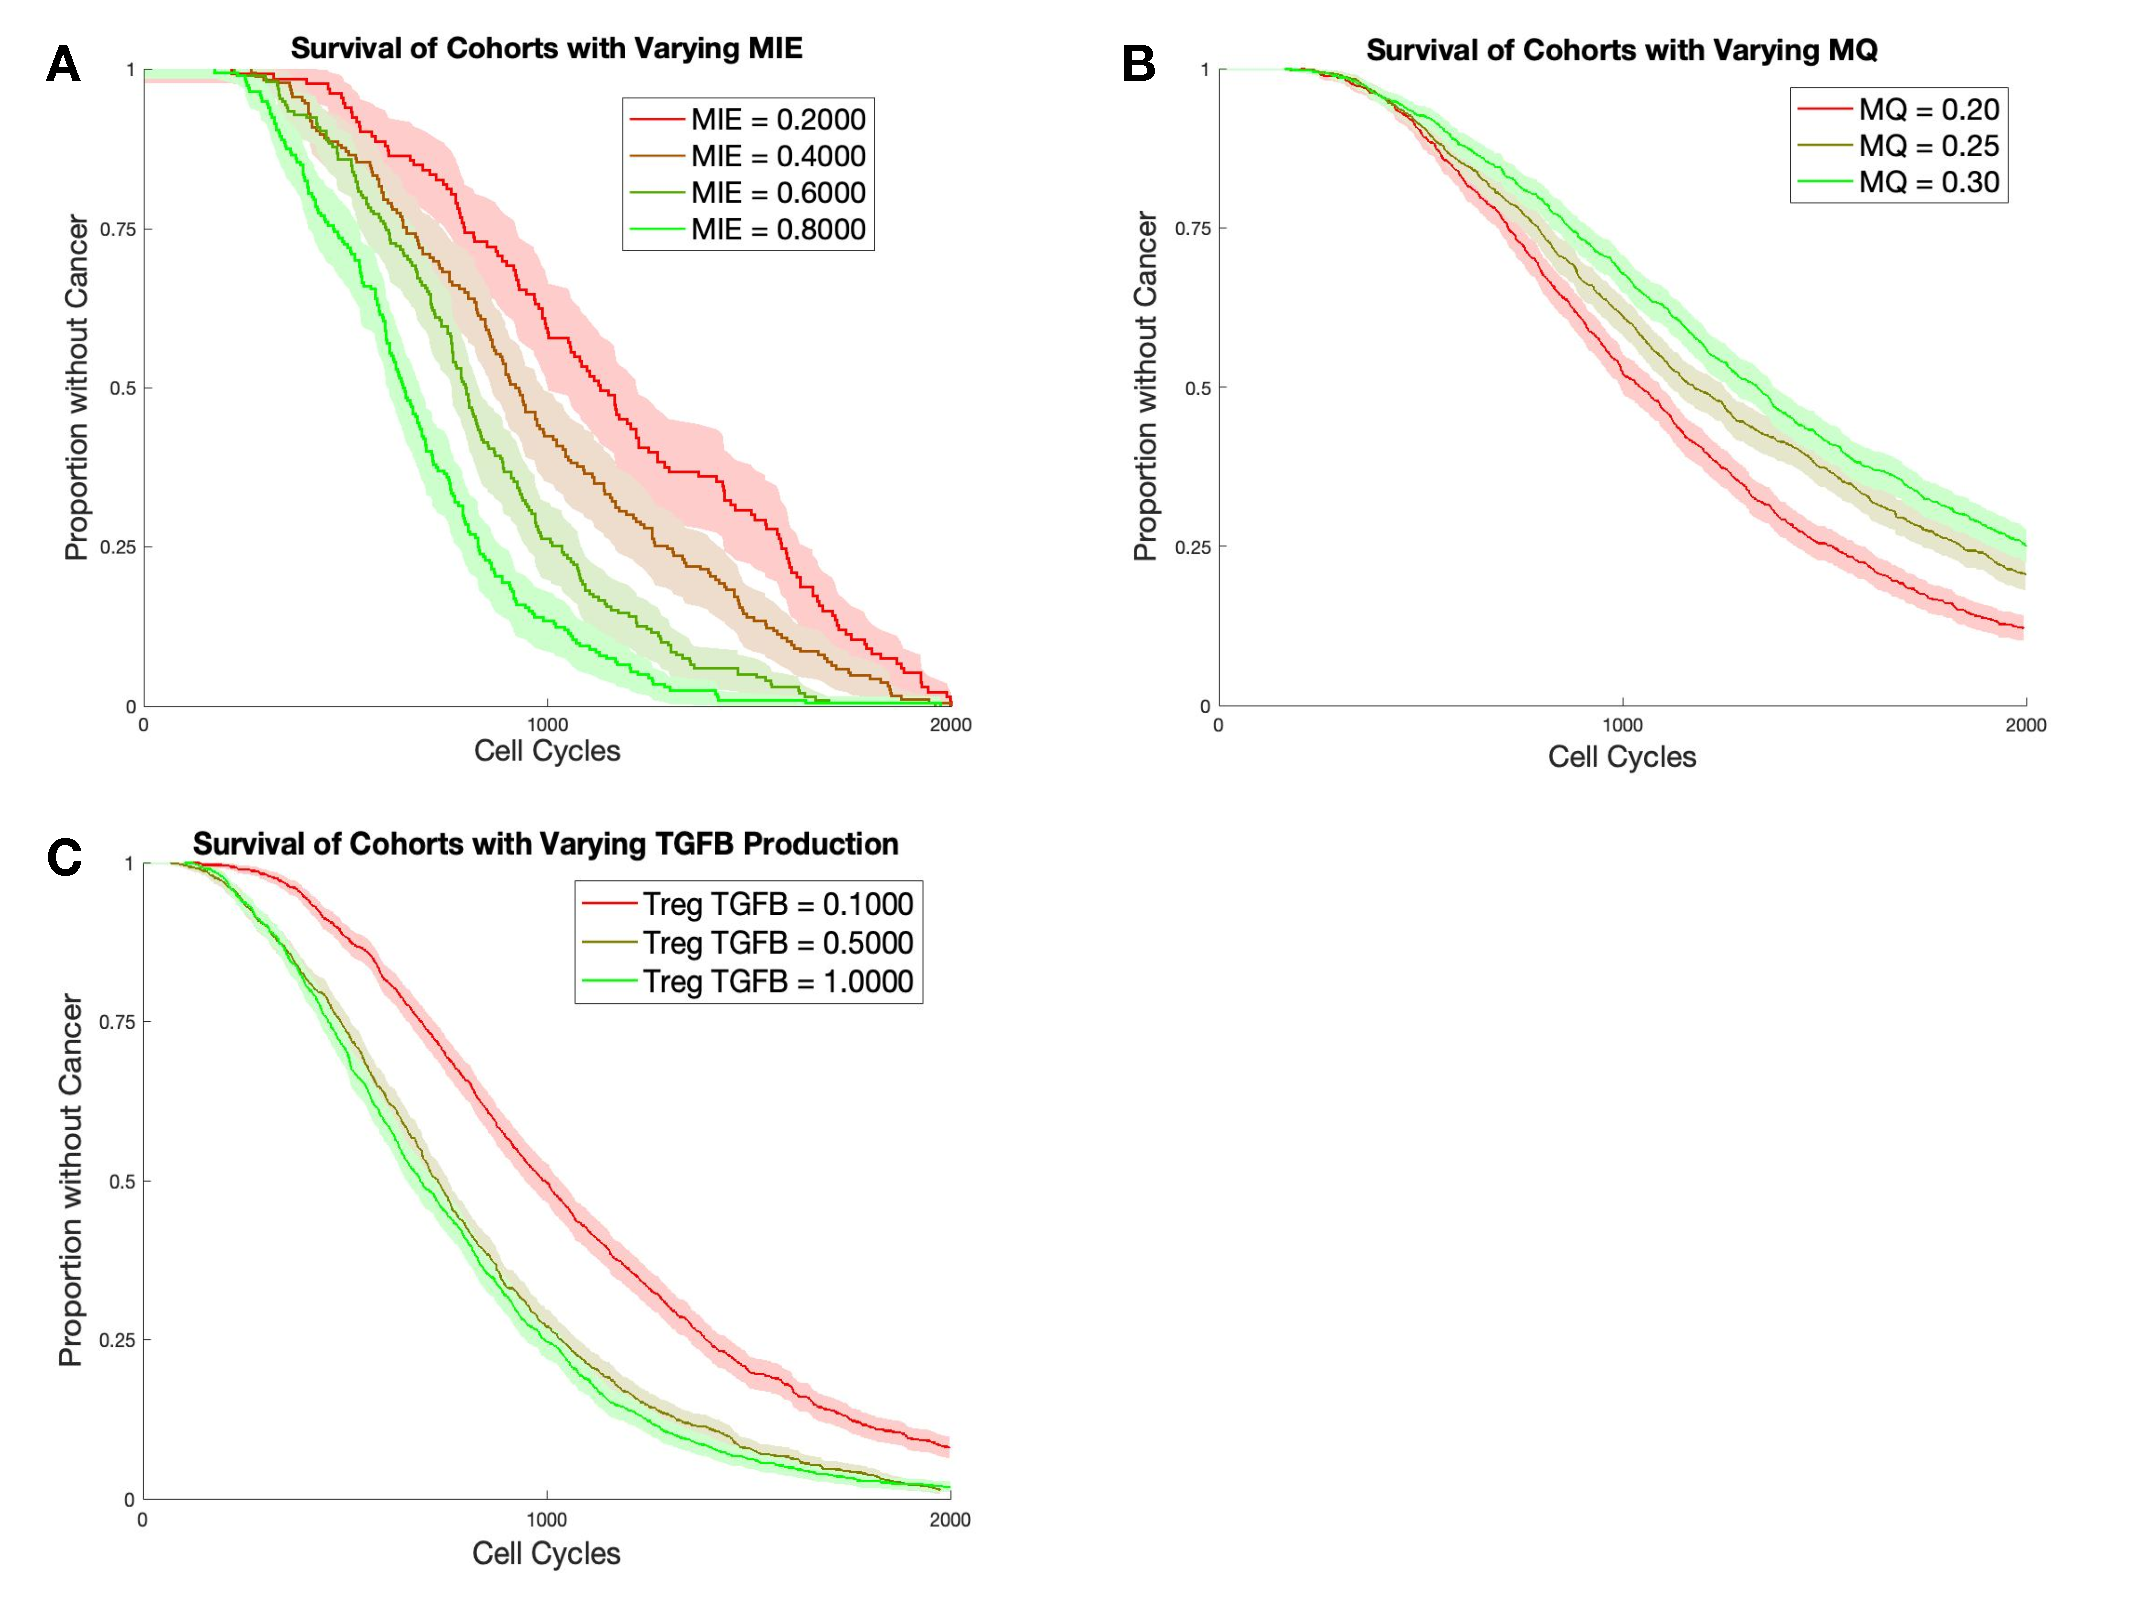
\includegraphics[width=\columnwidth]{Figure2/Figure2.pdf}}
\caption{A. Increasing MIE decreases Time to Cancer. 
B. Increasing MQ increases Time to Cancer.
C. Increasing Treg TGF-$\beta$ production results in decreased Time to Cancer.
%% {\color{red} Cox regression or KM test statistics to be computed to demonstrate the significance of this claim.}\newline
\newline
}
\label{fig:FirstSurvivalCurves}
\end{figure}

Second, as mesenchymal quiescence (MQ) increases, Time to Cancer increases.
This result will prove to be more interesting as this pattern is dependent on the other parameters in the model.
For now, what can be seen in Figure \ref{fig:FirstSurvivalCurves}B is that a slower proliferation for mesenchymal cells slows down cancer growth.
This is not as intuitive as it may sound because this decreased proliferation affects both mutated and non-mutated cells.
% It may be interesting to track how much MQ affects mutated vs. non-mutated cells throughout the time.
These results are summarized by Figure \ref{fig:FirstSurvivalCurves}B.

Third, TGF-$\beta$ can be varied in two ways: the production by mesenchymal cells and the production by Treg cells.
In Figure \ref{fig:FirstSurvivalCurves}C, the results of varying Treg TGF-$\beta$ production is shown, indicating that an increased Treg TGF-$\beta$ production leads to a shorter Time to Cancer.
This is expected as the two main ways in which TGF-$\beta$ influences the system is in recruitment of Treg cells and in pushing cells to a mesenchymal phenotype.
Treg cells are modeled as tumor-protective and thus increasing their number will naturally decrease Time to Cancer.
Mesenchymal cells are more likely to evade the immune system, so pushing the system towards an overall more mesenchymal phenotype will better protect the cancer and decrease the Time to Cancer.
% But what happens when MIE is really high to begin with so becoming mesenchymal mostly just makes you proliferate slower? Perhaps that can go in a supplementary figure?

\subsection{Key EMT regime maximizes cancer-free survival time under chronic inflammation}\label{KeyEMT}
Given the relevance of the inflammatory state of the tumor microenvironment (TME), we explore the effect of varying the inflammation state of the patient on survival.
In particular, some cohorts are assigned permanently low inflammation, others permanently high, and still others non-constant inflammatory schemes.
For those cohorts with a permanently high inflammatory state, the relationship between the mesenchymal parameters and the Time to Cancer is monotonic.
However, when there are periods of a low inflammatory state, then intriguingly the connection between MQ and Time to Cancer becomes concave down with a local maximum around 0.3.
What this indicates is that if the quiescence of mesenchymal cells can be controlled, then they could be manipulated in such a way as to increase the Time to Cancer and the time to death.
Furthermore, even if the patient is presenting a permanent high inflammatory state, medications could be prescribed which would lower the inflammatory state temporarily and thus create a similar cycling inflammatory regime which could be taken advantage of in the same way.
See Figure \ref{fig:VaryINFL_and_MesPars}C and Figure \ref{fig:VaryINFL_and_MesPars}D for a summary.

\begin{figure}[H]
\center
\frame{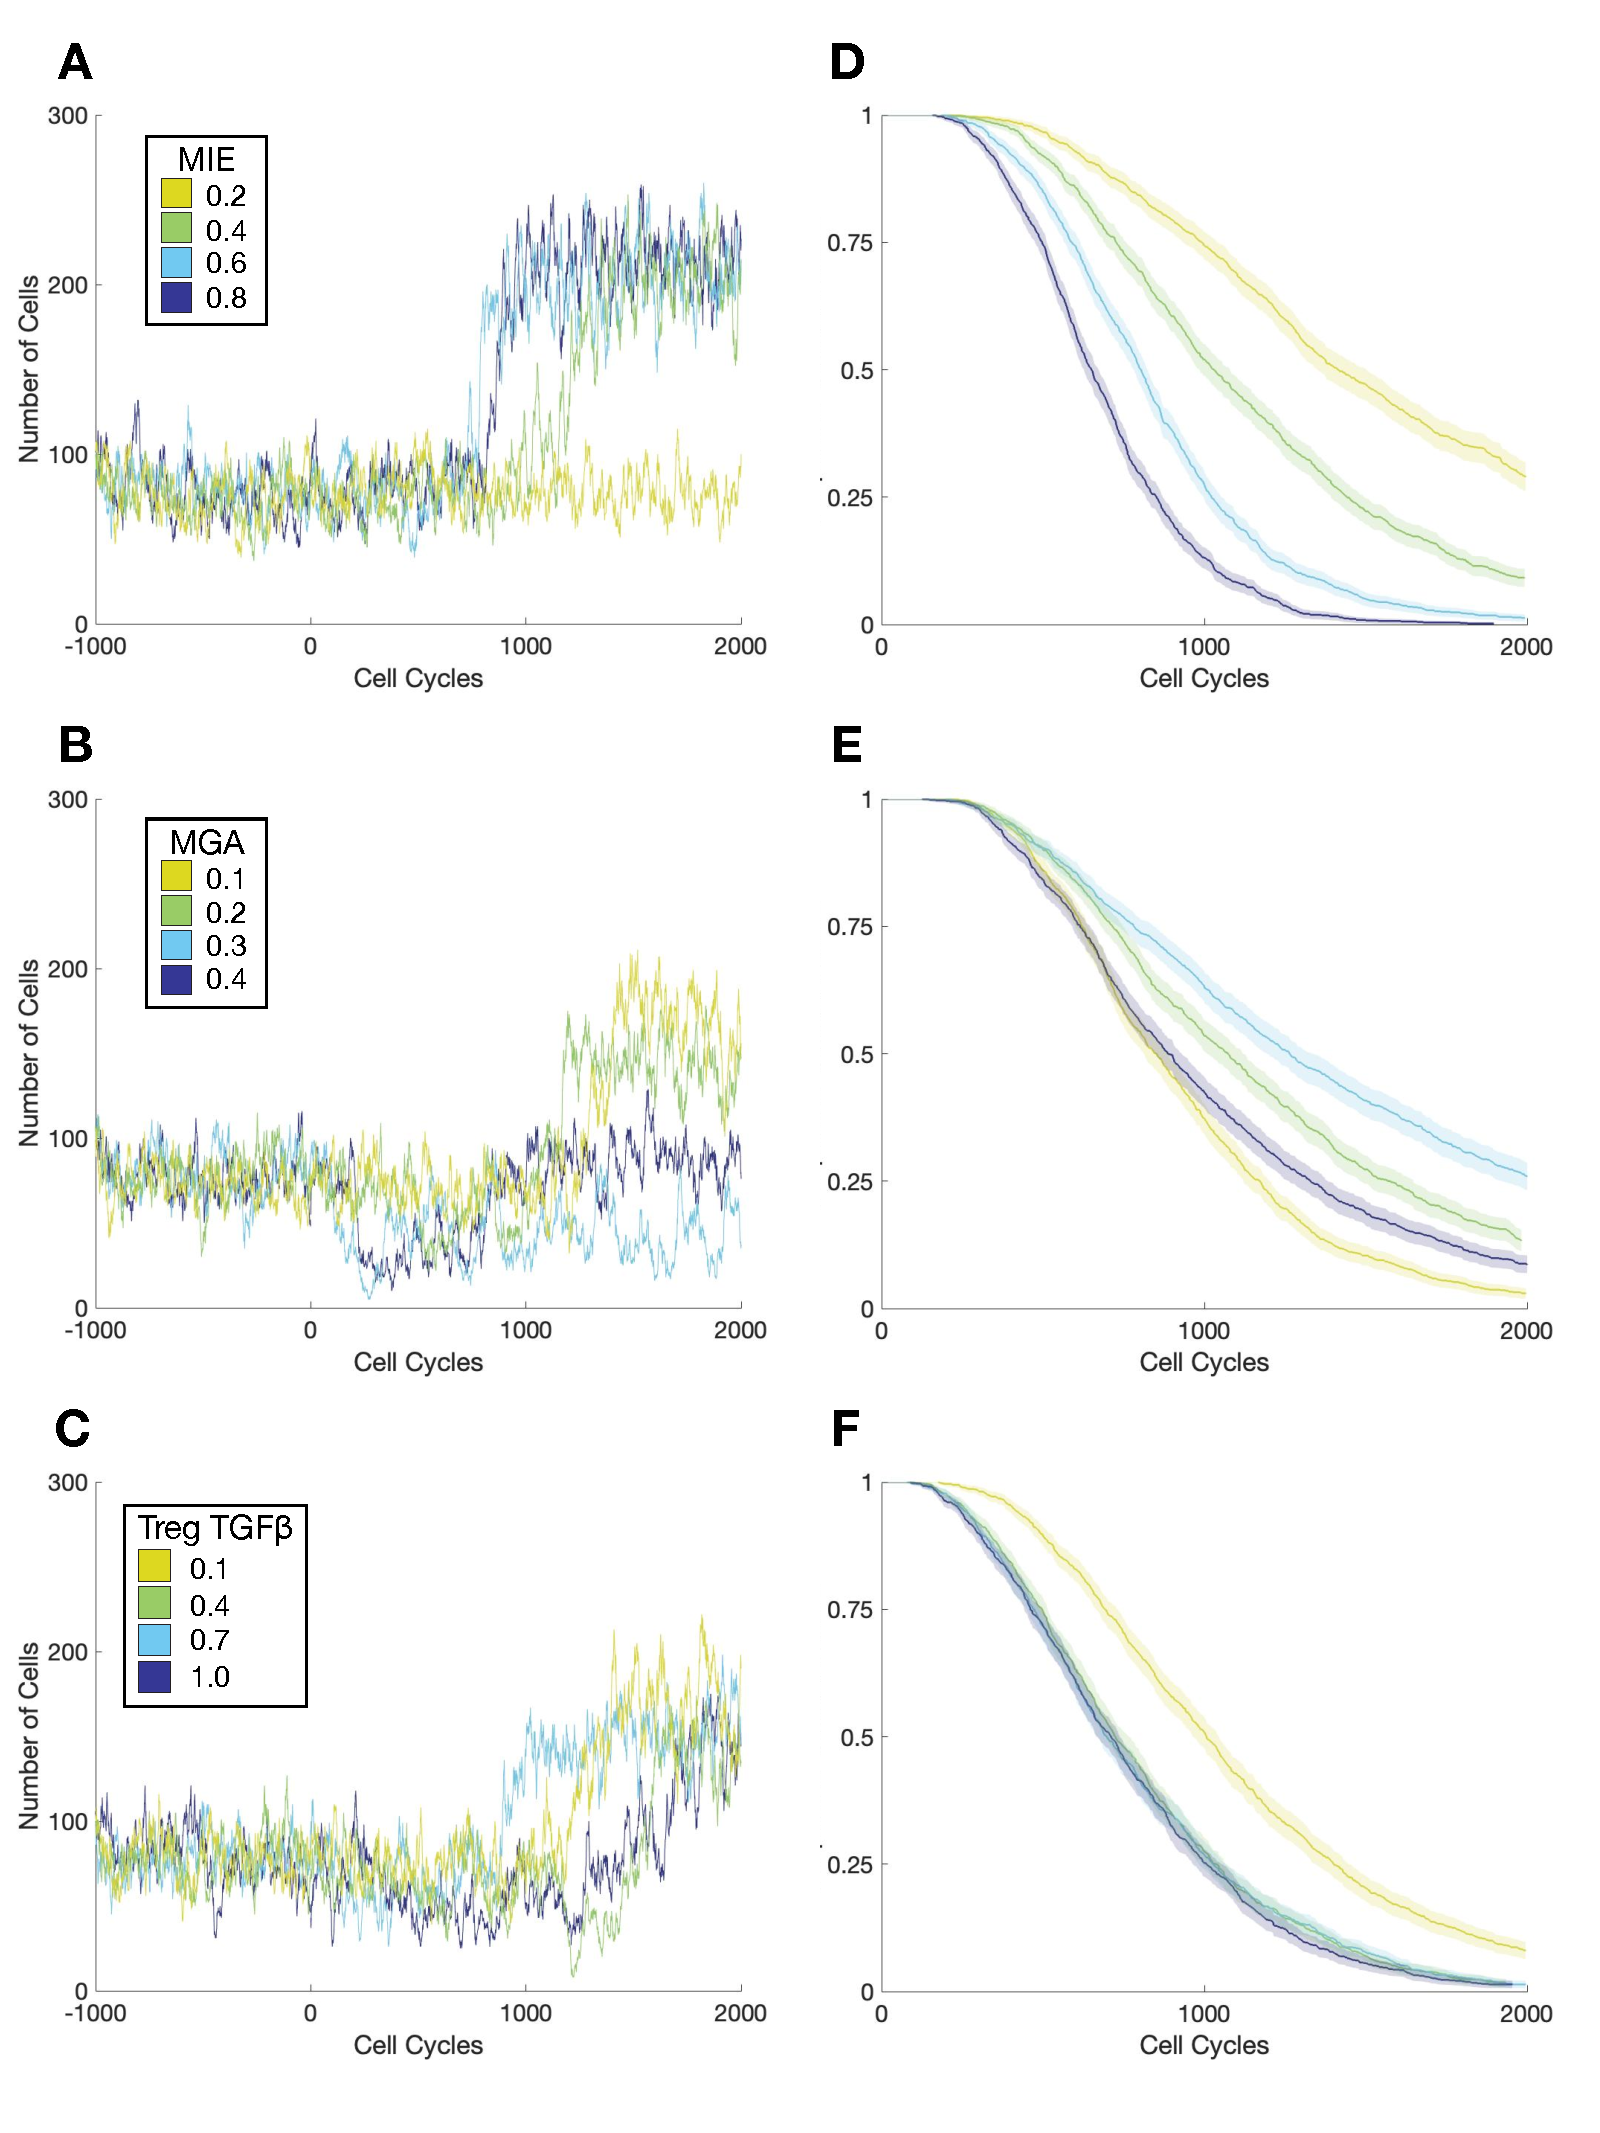
\includegraphics[width=\columnwidth]{Figure3/Figure3.pdf}}
\caption{A.Survival curves for various inflammation cycling schemes. In the top two plots, the Time to Cancer decreases as MIE increases. In the bottom plot, there is no significant difference in survival.
B. The average Time to Cancer for each cohort.
C. Survival curves for various inflammation cycling schemes. In the top two plots, the Time to Cancer reaches a maximum value somewhere near MQ = 0.3. In the bottom plot, there is no significant difference in survival.
D. The average Time to Cancer for each cohort.}
\label{fig:VaryINFL_and_MesPars}
\end{figure}

Contrast this with what happens when MIE is varied for different inflammation cycling schemes.
Regardless of the cycling scheme, the relationship between Time to Cancer and MIE is never non-monotonic.
In the case that the inflammatory state is permanently high, MIE has no significant effect on Time to Cancer.
On the other hand, when the patient experiences at least some time in a low inflammatory state, an increase in MIE results in a decrease in Time to Cancer.
This indicates that reducing the inflammatory state of the patient is a necessity for increasing survival, and once that has been achieved, even to a small degree, then therapies which reduce mesenchymal immune evasion will gain efficacy.
See Figure \ref{fig:VaryINFL_and_MesPars}A and Figure \ref{fig:VaryINFL_and_MesPars}B for a summary.

\subsection{Heat Map of MIE vs MQ}
To further draw out the contrast between these two mesenchymal properties, we compare Time to Cancer for many different pairs of values for MIE and MQ.
The heat map in Figure \ref{fig:MIEvsMQ} concisely encodes the relationships we have been observing in the previous sections.
Regardless of the value of MQ, increasing MIE leads to decreased Time to Cancer.
On the other hand, for any value of MIE, then there is an optimal MQ value in the sense that it results in the longest Time to Cancer.
It appears based on the plot that this value is around 0.28.

\begin{figure}[H]
\center
\frame{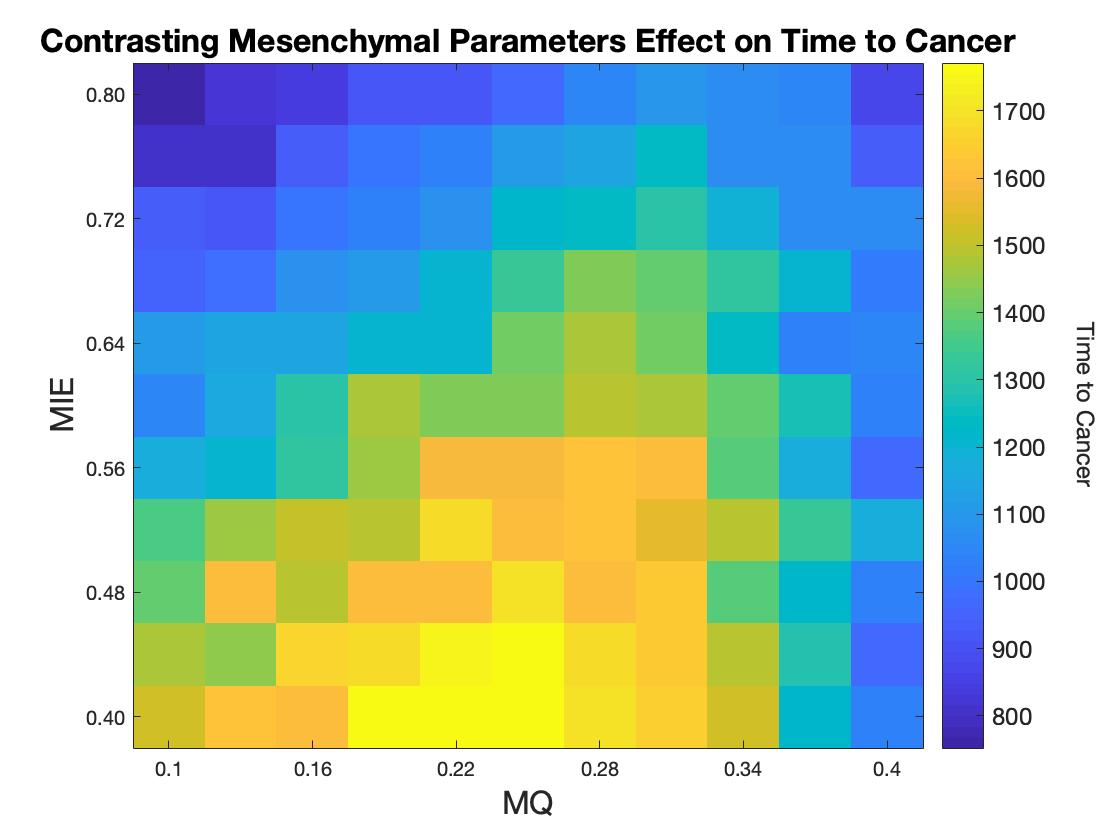
\includegraphics[width=\columnwidth]{Figure4/MIEvsMQ.jpg}}
\caption{Heat Map contrasting the effects of MIE and MQ on Time to Cancer. Increasing MIE always decreases Time to Cancer, but MQ is non-monotonically linked to Time to Cancer.}
\label{fig:MIEvsMQ}
\end{figure}

\section{Discussion}\label{Discussion}
This might actually be where I talk about the implication of the results from Section \ref{KeyEMT}.
In addition, I could discuss the implications from the TGF-$\beta$ section.
Any discussion on this topic, however, would need to acknowledge that regulation of TGF-$\beta$ might also have other, serious side effects, especially if the treatment is not local.
However, that might also be true for the inflammatory results.
In light of this, it might be good to include a new section on how TGF-$\beta$ production's influence on Time to Cancer is influenced by the inflammatory cycling scheme.

%%%%%%%%%%%%%%%%%%%%%%%
%                     CONCLUSION                      %
%%%%%%%%%%%%%%%%%%%%%%%

\section{Conclusion}\label{Conclusion}

\end{document}